\documentclass{beamer}

\mode<presentation> {
}

\title[]{Bayesian Clinical Trials} 
\subtitle{Sample Size for Binomial Proportions} 
\date{} 

\usepackage{graphicx} 
\usepackage{booktabs} 
\usepackage{longtable} 
 \usepackage{hyperref}


\usepackage{color}
\usepackage{fancyvrb}

\definecolor{shadecolor}{gray}{0.95}

\DefineShortVerb[commandchars=\\\{\}]{\|}
\DefineVerbatimEnvironment{Highlighting}{Verbatim}{commandchars=\\\{\}}
\newenvironment{Shaded}{}{}
\newcommand{\KeywordTok}[1]{\textcolor[rgb]{0.00,0.44,0.13}{\textbf{{#1}}}}
\newcommand{\DataTypeTok}[1]{\textcolor[rgb]{0.56,0.13,0.00}{{#1}}}
\newcommand{\DecValTok}[1]{\textcolor[rgb]{0.25,0.63,0.44}{{#1}}}
\newcommand{\BaseNTok}[1]{\textcolor[rgb]{0.25,0.63,0.44}{{#1}}}
\newcommand{\FloatTok}[1]{\textcolor[rgb]{0.25,0.63,0.44}{{#1}}}
\newcommand{\CharTok}[1]{\textcolor[rgb]{0.25,0.44,0.63}{{#1}}}
\newcommand{\StringTok}[1]{\textcolor[rgb]{0.25,0.44,0.63}{{#1}}}
\newcommand{\CommentTok}[1]{\textcolor[rgb]{0.38,0.63,0.69}{\textit{{#1}}}}
\newcommand{\OtherTok}[1]{\textcolor[rgb]{0.00,0.44,0.13}{{#1}}}
\newcommand{\AlertTok}[1]{\textcolor[rgb]{1.00,0.00,0.00}{\textbf{{#1}}}}
\newcommand{\FunctionTok}[1]{\textcolor[rgb]{0.02,0.16,0.49}{{#1}}}
\newcommand{\RegionMarkerTok}[1]{{#1}}
\newcommand{\ErrorTok}[1]{\textcolor[rgb]{1.00,0.00,0.00}{\textbf{{#1}}}}
\newcommand{\NormalTok}[1]{{#1}}

\hypersetup{breaklinks=true, pdfborder={0 0 0}}
\setlength{\parindent}{0pt}
\setlength{\parskip}{6pt plus 2pt minus 1pt}
\setlength{\emergencystretch}{3em}  
\setcounter{secnumdepth}{0}
%\EndDefineVerbatimEnvironment{Highlighting}


\begin{document}



\begin{frame}
\titlepage % Print the title page as the first slide
\end{frame}


\begin{frame}{Sample size based on interval widths}

What sample size is needed to provide sufficient information to specify
the true difference between two proportions \(\pi_{1}\) and \(\pi_{2}\)
to within a total 100(1-\(\alpha\)) interval width of given percentage
points (say \(w\))? \[
n=4Z_{1-\alpha/2}^2\frac{\left[\pi_{1}\left(1-\pi_{1}\right)+\pi_{2}\left(1-\pi_{2}\right)\right]}{w^2}
\]

This formula requires point estimates of \(\pi_{1}\) and \(\pi_{2}\)
while a better summary of the available information is a distribution
over a range of values.

\end{frame}





\begin{frame}{Bayesian approach}

Let \(\theta\) in \(\Theta\) the parameter of interest. We recall that
the posterior distribution is \[
f\left(\theta\vert x\right)=\frac{L\left(x\vert \theta\right)g\left(\theta\right)}{\int_\Theta L\left(x\vert\theta\right)g\left(\theta\right) d\theta}
\] and depends on the data \(x\), which is of course unknown at the
planning stages of the experiment. The pre-posterior predictive
distribution is defined by the denominator in Bayes' Theorem which
decribes the expectation of the likelihood function over the prior
distribution: \[
f\left(x\right)=\int_\Theta L\left(x\vert \theta\right)g\left(\theta\right) d\theta
\]

\end{frame}



\begin{frame}{Bayesian approach}

We refer to as fully Bayesian (FB) approach when
\(g\left(\theta\right)\) represents the true prior information in both
posterior and pre-posterior predictive distributions

We refer to as mixed Bayesian/likelihood (MBL) approach when
\(g\left(\theta\right)\) represents the true prior information in
posterior distribution but substitutes a uniform density in
pre-posterior.

Typically, we wish a highest posterior density (HPD) or other posterior
credible interval of length \(l\) that covers \(\theta\) with
probability \((1-\alpha)\). HPD are optimal in the sense that they lead
to the smallest sample sizes for any given coverage.

\end{frame}

\begin{frame}{Criteria based on HPD (Joseph et al, 1997)}

\begin{itemize}
\itemsep1pt\parskip0pt\parsep0pt
\item
  ACC: controls the coverage rate of fixed length credible intervals
  over the predictive distribution of the data
\item
  ALC: controls the length of credible intervals with a fixed coverage
  rate over the predictive distribution of the data.
\item
  WOC: guarantees that the desired coverage rate and interval length
  over all (or a subset of) possible datasets.
\end{itemize}

\end{frame}




\begin{frame}{Average Coverage Criterion (ACC)}

The ACC sample size is the smallest integer such that for a fixed
nominal interval length \(l\) the expected coverage level is at least
\(1 - \alpha\), where expectation is taken over the marginal
distribution of \(x\): \[
\int \left(\int_{a\left(x,n\right)}^{a\left(x,n\right)+l} f\left(\theta\vert x\right) d\theta\right) f\left(x\right) dx \ge 1-\alpha 
\]

where \(a\left(x,n\right)\) is the lower limit of the HPD interval of
length \(l\) for the posterior density.

\end{frame}


\begin{frame}{Average Length Criterion (ALC)}

The ALC sample size is the smallest integer such that for a fixed
nominal coverage level \(1 - \alpha\) the expected length is at most
\(l\), where expectation is taken over the marginal distribution of
\(x\). The ALC has a two-step formula. The first step is to find the HPD
length \(l'\left(x,n\right)\) that satisfies \[
\int_{a\left(x,n\right)}^{a\left(x,n\right)+l'\left(x,n\right)} f\left(\theta\vert x\right) d\theta=1-\alpha
\] Then choose the minimum \(n\) that satisfies: \[
\int  l'\left(x,n\right) f\left(x\right) dx \le l
\]

\end{frame}




\begin{frame}{Worst Outcome Criterion (WOC)}

The WOC sample size is determined by the smallest integer \(n\) such
that \[
\inf \left(\int_{a\left(x,n\right)}^{a\left(x,n\right)+l} f\left(\theta\vert x\right) d\theta\right) \ge 1-\alpha 
\]

\end{frame}




\begin{frame}{Comparison between ALC, ACC and WOC (Cao et al, 2009)}

\begin{itemize}
\item
  Because most researchers tend to report the length of the confidence
  interval of a fixed coverage, instead of the coverage of the interval
  of a fixed length, the ALC is more conventional than the ACC.
\item
  WOC provides a conservative sample size and can give more assurance
  than the ``average'' assurances provided by the ACC and ALC criteria.
\item
  When a posterior density has the common density shape of concave flat
  tails and convex steep center, the nominal coverage \(1-\alpha\) will
  determine the relative difference between the ALC sample size and the
  ACC sample size. A ``small'' \(\alpha\) implies that ACC needs a
  larger sample size than the ALC. It is the opposite for ``bigger''
  \(\alpha\).
\end{itemize}

\end{frame}



\begin{frame}{The difference of two binomial proportions}

Let \(x_{1}\) and \(x_{2}\) be the total number of successes out of
\(n_{1}\) and \(n_{2}\) trials from independent binomial experiments
with parameters \(\pi_{1}\) and \(\pi_{2}\), respectively. We can choose
two independent beta priors
\(g\left(\pi_{1}\right)=Beta\left(c_{1},d_{1}\right)=B\left(c_{1},d_{1}\right)^{-1}\pi_{1}^{c_{1}-1}\left(1-\pi_{1}\right)^{d_{1}-1}\)
\(g\left(\pi_{2}\right)=Beta\left(c_{2},d_{2}\right)=B\left(c_{2},d_{2}\right)^{-1}\pi_{2}^{c_{2}-1}\left(1-\pi_{2}\right)^{d_{2}-1}\)

for \(\pi_{1}\) and \(\pi_{2}\), respectively - each conjugate to the
binomial likelihood - so the posterior distribution is the product of
two Beta distributions:



\begin{align}
& f\left(\pi_{1},\pi_{2}\right\vert x_{1},x_{2},n_{1},n_{2})= \\
& = \frac {\prod_{i=1}^2 {\pi_{i}^{c_{i}+x_{i}-1}\left(1-\pi_{i}\right)^{d_{i}+n_{i}-x_{i}-1}}} {B\left(c_{1}+x_{1},d_{1}+n_{1}-x_{1}\right)B\left(c_{2}+x_{2},d_{2}+n_{2}-x_{2}\right)}
\end{align}


\end{frame}


\begin{frame}{The difference of two binomial proportions}

and the predictive distribution is the product of two betabinomial
distributions: 
\begin{align}
& p\left(x_{1},x_{2}\right)=\\
&=\prod_{i=1}^2 {\left[B\left(c_{i}+x_{i},d_{i}+n_{i}-x_{i}\right)B\left(c_{i},d_{i}\right)\right]^{-1}\pi_{i}^{c_{i}+x_{i}-1}\left(1-\pi_{i}\right)^{d_{i}+n_{i}-x_{i}-1} }
\end{align}



We make a change of variable as \(\theta=\pi_{2}-\pi_{1}\) and the
posterior becomes:


\begin{align}
& f\left(\pi_{1},\theta\vert x_{1},x_{2},n_{1},n_{2}\right)\propto \\
& \propto \pi_{1}^{c_{1}+x_{1}-1}\left(1-\pi_{1}\right)^{d_{1}+n_{1}-x_{1}-1} \left(\pi_{1}-\theta\right)^{c_{2}+x_{2}-1}\left(1-\pi_{1}+\theta\right)^{d_{2}+n_{2}-x_{2}-1}
\end{align}


It follows that the marginal posterior distribution of \(\theta\) is

\[
f\left(\theta\vert x_{1},x_{2},n_{1},n_{2}\right)=\int_{\max{0,\theta}}^{\min{\theta+1,1}} f\left(\pi_{1},\theta\vert x_{1},x_{2},n_{1},n_{2}\right) d\pi_{1}
\]

For ease, assume \(n_{1}=n_{2}=n\)

\end{frame}


\begin{frame}{The difference of two binomial proportions}

\begin{itemize}
\itemsep1pt\parskip0pt\parsep0pt
\item
  ACC sample size for \(\theta\) is the minimum n:
\end{itemize}

\[
\sum_{x_{1}=0}^{n} \sum_{x_{2}=0}^{n} \int_{a\left(x_{1},x_{2}\right)}^{a\left(x_{1},x_{2}\right)+l} f\left(\theta\vert x_{1},x_{2},n\right)d\theta\phantom{0}p\left(x_{1},x_{2}\right) \ge 1-\alpha 
\]

\begin{itemize}
\itemsep1pt\parskip0pt\parsep0pt
\item
  ALC sample size for \(\theta\) is the minimum n:
\end{itemize}

\[
\sum_{x_{1}=0}^{n} \sum_{x_{2}=0}^{n} l'\left(x_{1},x_{2}\right) p\left(x_{1},x_{2}\right) \le l 
\]

where \(l'\left(x_{1},x_{2}\right)\) is the HPD length that satisfies:

\[
\int_{a\left(x_{1},x_{2}\right)}^{a\left(x_{1},x_{2}\right)+l'\left(x_{1},x_{2}\right)} f\left(\theta\vert x_{1},x_{2},n\right)d\theta =1-\alpha
\]

\end{frame}



\begin{frame}{The difference of two binomial proportions}

\begin{itemize}
\itemsep1pt\parskip0pt\parsep0pt
\item
  WOC sample size for \(\theta\) is the minimum n:
\end{itemize}

\[
\int_{a\left(x_{1}^{*},x_{2}^{*}\right)}^{a\left(x_{1}^{*},x_{2}^{*}\right)+l} f\left(\theta\vert x_{1}^{*},x_{2}^{*},n\right)d\theta \ge 1-\alpha
\]

where \(x_{1}^{*}\) and \(x_{2}^{*}\) are the numbers of successes that
maximize the length of the HPD interval.

\end{frame}




\begin{frame}{Example (Joseph et al, 1997)}

Consider a clinical trial planned to study the rates of myocardial
infraction (MI) for patients with acute unstable angina pectoris
following two different study regimens.

A previous study reported MI rates in aspirin group=4/121, in aspirin
and heparin combination group= 2/122 and 14/118 in placebo group.

Using the above prior information, what sample size do we need so that
the 95\% HPD interval for the difference in rates between aspirin and
aspirin with heparin has a total length of 3 percentage points?

\end{frame}



\begin{frame}{Example (Joseph et al, 1997)}

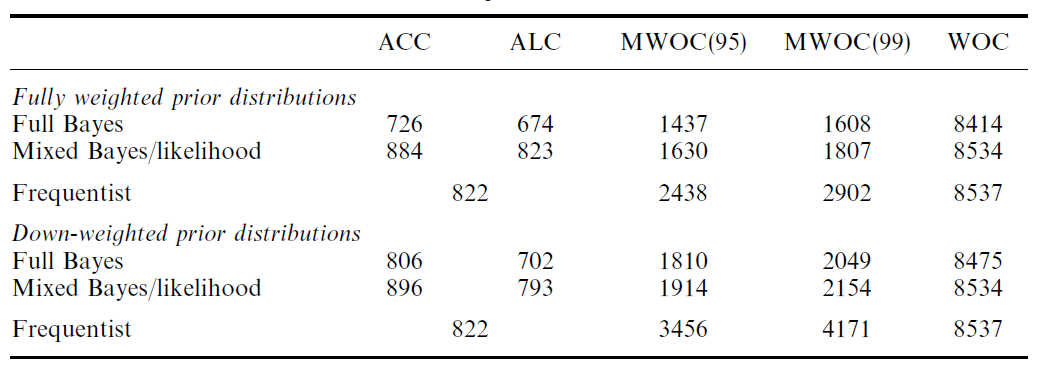
\includegraphics[scale=0.4]{images/Figure.png}

\end{frame}

\begin{frame}[fragile]{R code}

\begin{Shaded}
\begin{Highlighting}[]
\KeywordTok{suppressWarnings}\NormalTok{(}\KeywordTok{library}\NormalTok{(SampleSizeProportions))}
\NormalTok{len<-}\FloatTok{0.03}
\NormalTok{level<-}\FloatTok{0.95}
\NormalTok{a<-}\KeywordTok{matrix}\NormalTok{(}\DecValTok{0}\NormalTok{,}\DecValTok{1}\NormalTok{,}\DecValTok{4}\NormalTok{)}
\KeywordTok{colnames}\NormalTok{(a)<-}\KeywordTok{c}\NormalTok{(}\StringTok{"ACC"}\NormalTok{,}\StringTok{"ALC"}\NormalTok{,}\StringTok{"WOC"}\NormalTok{,}\StringTok{"frequentist"}\NormalTok{)}
\NormalTok{a[}\DecValTok{1}\NormalTok{]<-}\KeywordTok{propdiff.acc}\NormalTok{(}\DataTypeTok{len=}\NormalTok{len, }\DecValTok{4}\NormalTok{, }\DecValTok{117}\NormalTok{, }\DecValTok{2}\NormalTok{, }\DecValTok{120}\NormalTok{, }\DataTypeTok{level =} \NormalTok{level, }\DataTypeTok{equal =} \OtherTok{TRUE}\NormalTok{, }\DataTypeTok{m =} \DecValTok{10000}\NormalTok{, }\DataTypeTok{mcs =} \DecValTok{3}\NormalTok{)[}\DecValTok{1}\NormalTok{]}
\NormalTok{a[}\DecValTok{2}\NormalTok{]<-}\KeywordTok{propdiff.alc}\NormalTok{(}\DataTypeTok{len=}\NormalTok{len, }\DecValTok{4}\NormalTok{, }\DecValTok{117}\NormalTok{, }\DecValTok{2}\NormalTok{, }\DecValTok{120}\NormalTok{, }\DataTypeTok{level =} \NormalTok{level, }\DataTypeTok{equal =} \OtherTok{TRUE}\NormalTok{, }\DataTypeTok{m =} \DecValTok{10000}\NormalTok{, }\DataTypeTok{mcs =} \DecValTok{3}\NormalTok{)[}\DecValTok{1}\NormalTok{]}
\NormalTok{a[}\DecValTok{3}\NormalTok{]<-}\KeywordTok{propdiff.woc}\NormalTok{(}\DataTypeTok{len=}\NormalTok{len, }\DecValTok{4}\NormalTok{, }\DecValTok{117}\NormalTok{, }\DecValTok{2}\NormalTok{, }\DecValTok{120}\NormalTok{, }\DataTypeTok{level =} \NormalTok{level, }\DataTypeTok{equal =} \OtherTok{TRUE}\NormalTok{)[}\DecValTok{1}\NormalTok{]}
\NormalTok{a[}\DecValTok{4}\NormalTok{]<-}\KeywordTok{propdiff.freq}\NormalTok{(}\DataTypeTok{len=}\NormalTok{len, }\DataTypeTok{p1=}\FloatTok{0.016}\NormalTok{, }\DataTypeTok{p2=}\FloatTok{0.033}\NormalTok{, }\DataTypeTok{level =} \NormalTok{level)[}\DecValTok{1}\NormalTok{]}
\KeywordTok{print}\NormalTok{(a)}
\end{Highlighting}
\end{Shaded}

\end{frame}

\begin{frame}{References}

\begin{itemize}
\item
  Joseph L, du Berger R, Bélisle P. Bayesian and mixed
  Bayesian/likelihood criteria for sample size determination. Stat Med
  1997; 16(7): 769-781.
\item
  Cao J, Lee JJ, Alber S. Comparison of Bayesian sample size criteria:
  ACC, ALC, and WOC. J Stat Plan Inference 2009; 139(12):4111-4122.
\end{itemize}

\end{frame}


\end{document}